\chapter{GEOREFERENSI DATA RASTER}

Jika kita mempunyai sebuah data raster yang berasal dari hasil \textit{scanning} peta, foto udara, dan citra satelit yang belum berisi informasi yang menunjukkan referensi spasial. Kemudian kita ingin melakukan digitasi berdasarkan data \textit{raster} tersebut. Maka yang diperlukan adalah membuat peta hasil \textit{scan} tersebut mempunyai sistem koordinat dengan melakukan koreksi geometrik yaitu proses \textit{georeference}. \textit{Georeference} merupakan proses transformasi koordinat pada data \textit{raster} dari koordinat \textit{scanner} ke koordinat \textit{real-world}.

Selain foto udara dan citra satelit, data \textit{raster} bisa diperoleh melalui hasil \textit{scanning} peta analog. Peta yang baik pasti memiliki informasi koordinat geografis yang ditunjukkan dengan \textit{Grid} pada peta tersebut.

Pada Bab ini, akan dipelajari bagaimana melakukan georeferensi terhadap data \textit{raster} hasil \textit{scanning} peta analog. Untuk memulai proses georeferensi tahapan-tahapan yang dilakukan adalah sebagai berikut :

\begin{enumerate}[1.]

  \item Pada jendela utama Quantum GIS, klik \verb|Raster > Georeferencer > Georeferencer|, bila menu tersebut tidak muncul seperti gambar \ref{fig:georefmenunotexists}.
  
  \begin{figure}[H]
    \centering
    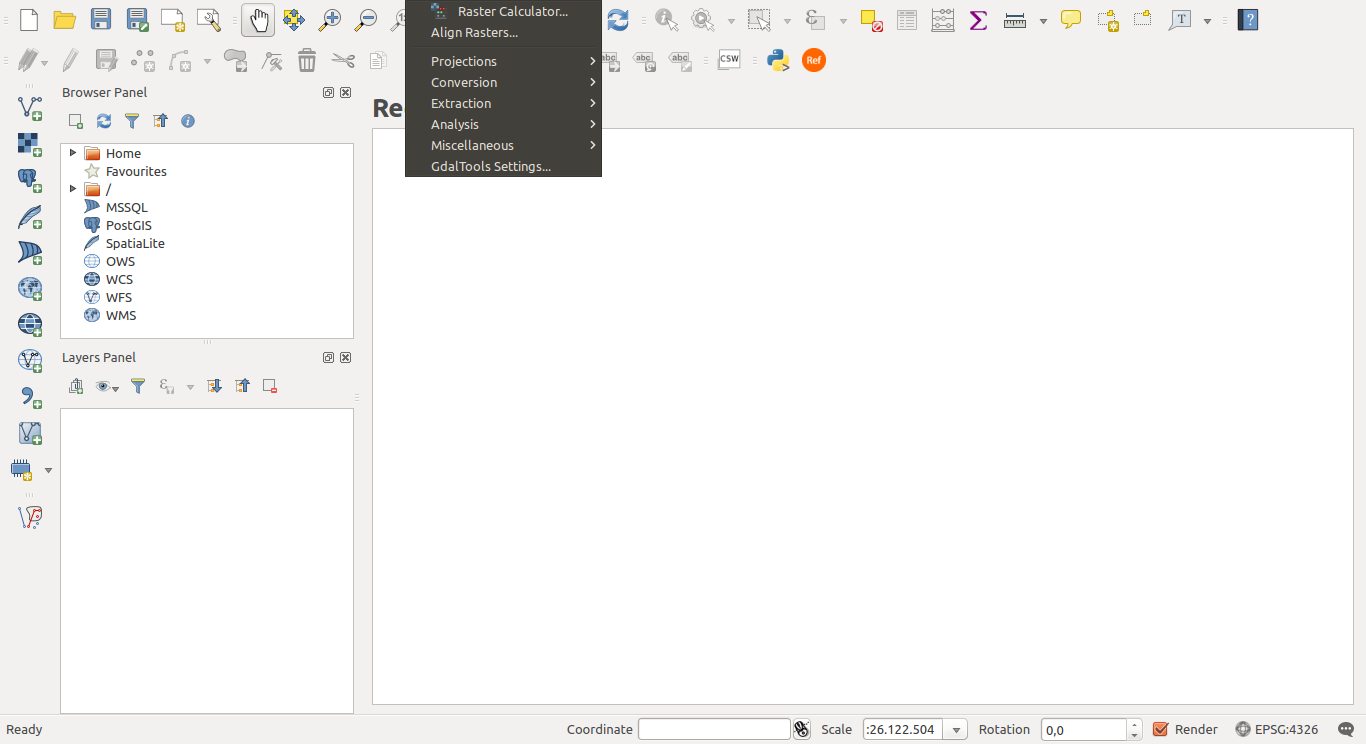
\includegraphics[width=1\textwidth]{./resources/018-menu-georeference-not-exists}
    \caption{Menu \textit{Georeference} tidak muncul}
    \label{fig:georefmenunotexists}
  \end{figure}
  
  Maka perlu memasangkan (\textit{install}) \textit{plugins} untuk \textit{georeferencer} terlebih dahulu dengan cara klik menu \verb|Plugins > Manage and Install Plugins...| sehingga muncul jendela pada gambar \ref{fig:pluginswin}.
  
  \begin{figure}[H]
    \centering
    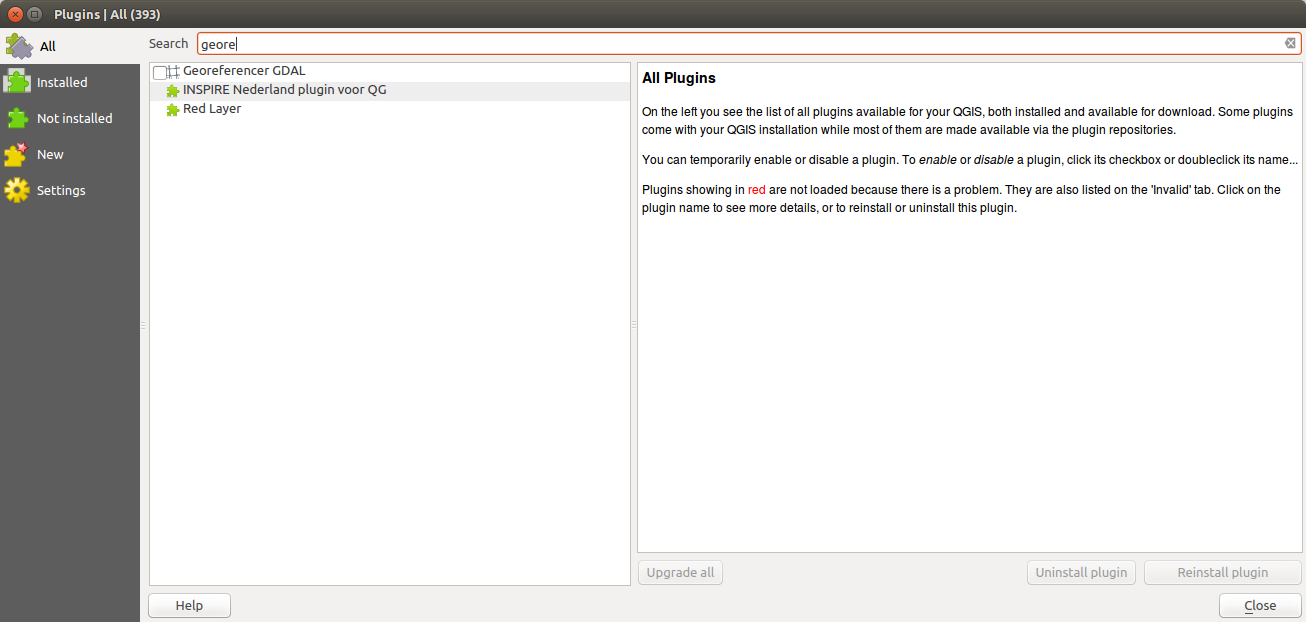
\includegraphics[width=1\textwidth]{./resources/020-pluginswin}
    \caption{Jendela \textit{Plugins}}
    \label{fig:pluginswin}
  \end{figure}
  
  sebelum jendela \textit{plugins} tersebut muncul, mungkin akan terlihat sebuah proses \textit{fetching repo} seperti pada gambar \ref{fig:fetchingrepo}.
  
  \begin{figure}[H]
    \centering
    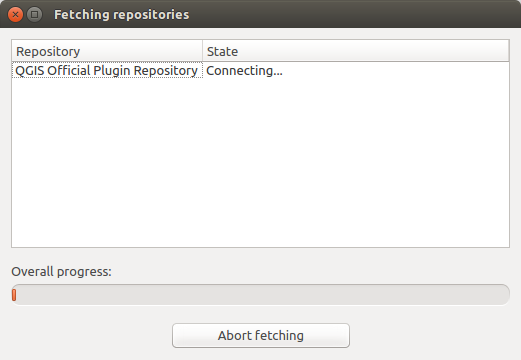
\includegraphics[width=1\textwidth]{./resources/019-fetching-repo}
    \caption{Jendela \textit{Fetching Repository}}
    \label{fig:fetchingrepo}
  \end{figure}
  
  Pada jendela \textit{plugins}, terdapat bagian \textit{search} untuk mempermudah mencari \textit{plugins} yang akan dipasang, ketikkan \verb|georeferencer| di kotak tersebut, lalu pilih tanda centang di sebelahnya. Bila belum terpasang, klik \verb|install plugin| di bagian jendela paling kanan bawah. Setelah selesai, maka akan muncul menu \verb|Georeferencer| pada menu \verb|Raster| seperti pada gambar \ref{fig:georefmenuexists}
  
  \begin{figure}[H]
    \centering
    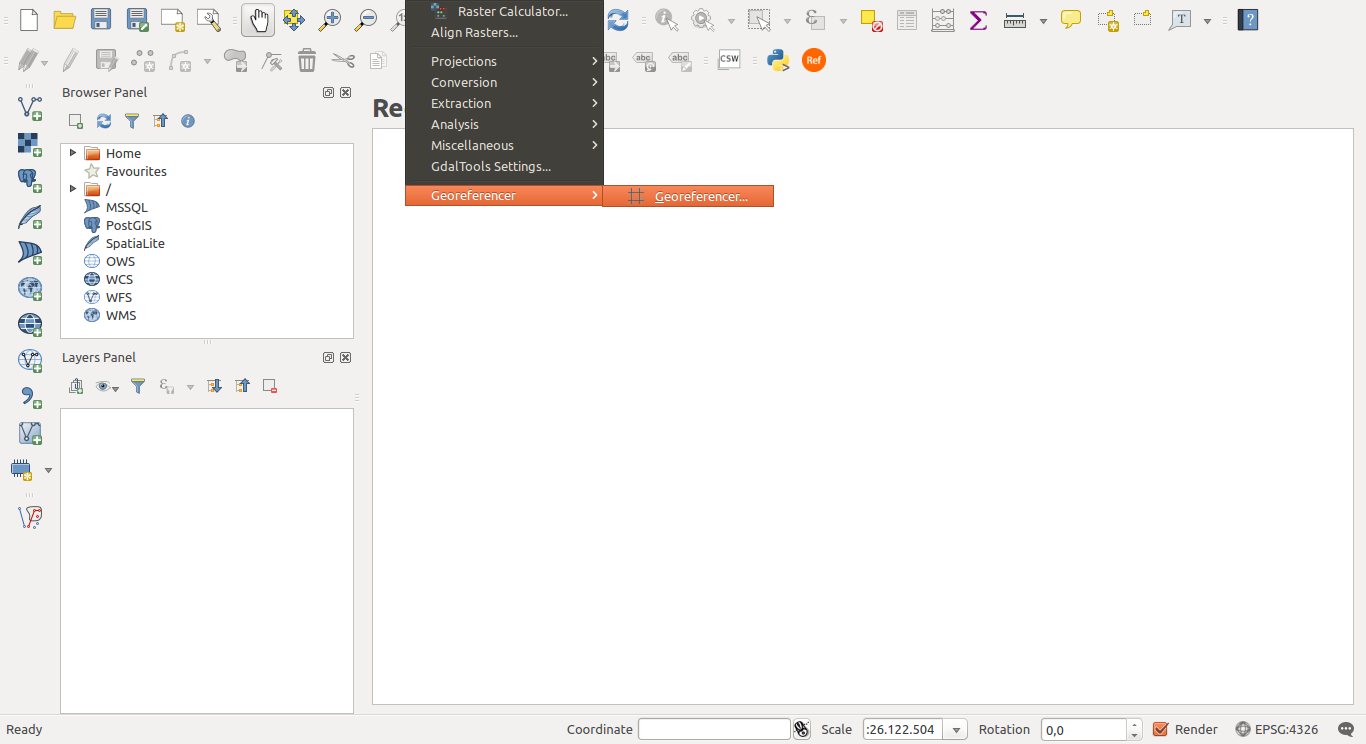
\includegraphics[width=1\textwidth]{./resources/021-georef-menu-exists}
    \caption{Menu \textit{Georeferencer} Muncul}
    \label{fig:georefmenuexists}
  \end{figure}
  
  Setelah memilih menu \verb|georeferencer| maka akan muncul jendela seperti pada gambar \ref{fig:georefwin}.
  
  \begin{figure}[H]
    \centering
    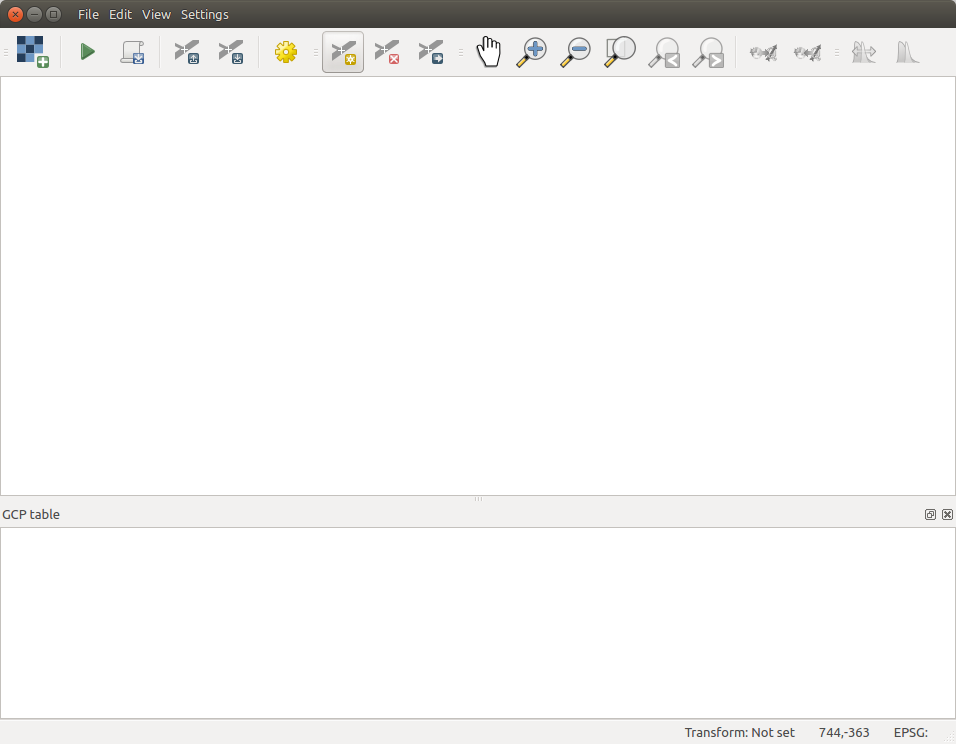
\includegraphics[width=1\textwidth]{./resources/022-georef-win}
    \caption{Jendela \textit{Georeferencer}}
    \label{fig:georefwin}
  \end{figure}
  
  \item Pada jendela \textit{georeferences}, klik \verb|File > Open Raster|. Kemudian pilih peta yang akan di georeferensi. Biasanya dalam bentuk JPG, atau GIF, atau bentuk format gambar yang lain yang didukung. Setelah membuka file \textit{raster} / gambar yang akan di georeferensikan, maka akan muncul gambar yang siap untuk diberikan koordinatnya seperti pada gambar \ref{fig:georeftif}
  
  \begin{figure}[H]
    \centering
    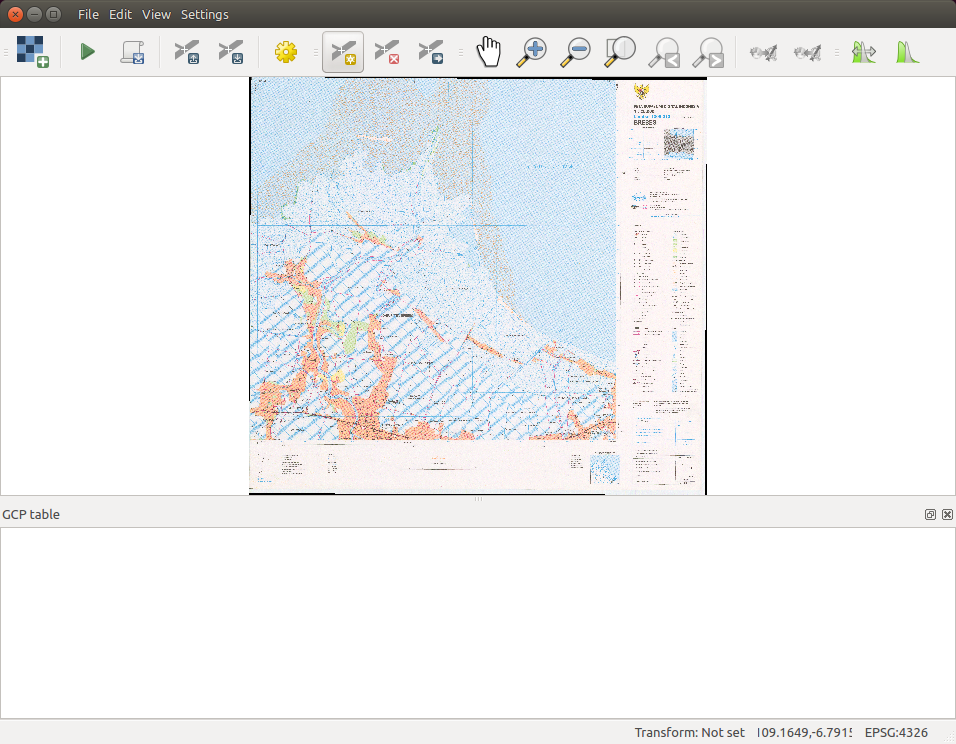
\includegraphics[width=1\textwidth]{./resources/023-georef-tif}
    \caption{\textit{File} TIF Yang Siap Untuk Digeoreferensikan}
    \label{fig:georeftif}
  \end{figure}
  
  Untuk memetakan 1 (satu) Kabupaten Brebes, sebetulnya lebih cocok menggunakan sistem koordinat terproyeksi seperti UTM, maka sumber data peta hasil \textit{scan} akan lebih memudahkan apabila terdapat informasi sebagaimana ditujukan pada gambar \ref{fig:refutm}.
  
  \begin{figure}[H]
    \centering
    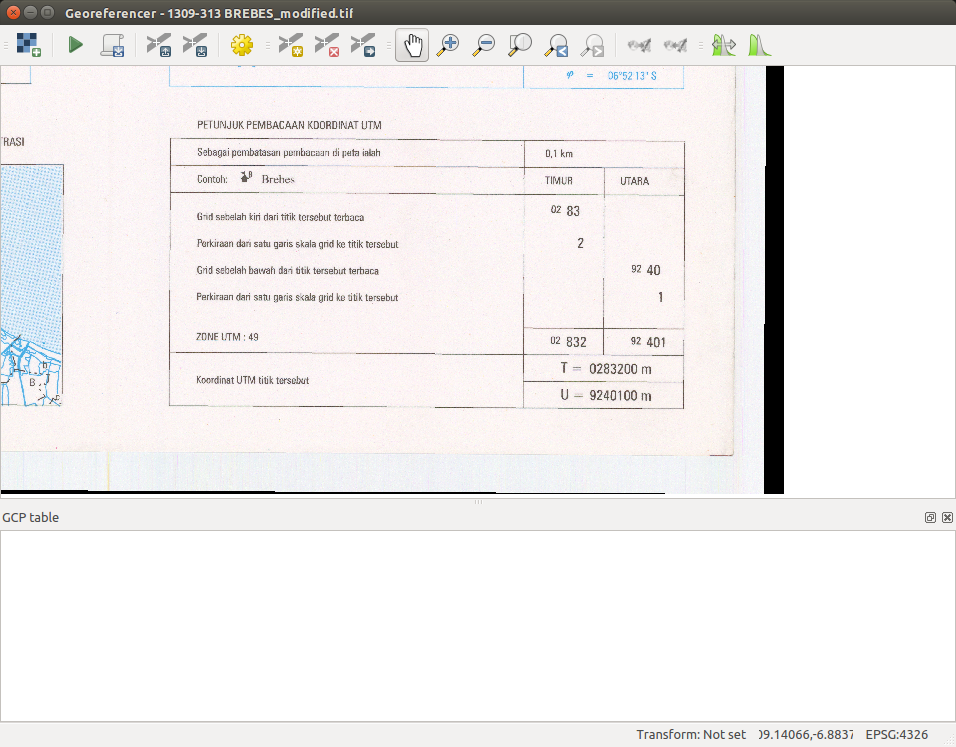
\includegraphics[width=1\textwidth]{./resources/024-utmpeta}
    \caption{Informasi Referensi UTM}
    \label{fig:refutm}
  \end{figure}
  
  Jika diperhatikan, maka peta hasil \textit{scan} tersebut masuk ke dalam zona 49. Karena informasi yang ditunjukkan oleh peta berada pada koordinat geografis S (\textit{South}) maka dapat dipastikan bahwa \textit{grid} peta tersebut berada pada zona 49S.
  
  Sebelum menentukan titik ikat, maka diperlukan proyeksi yang tepat terlebih dahulu dengan klik menu \verb|Settings > Transformation Settings...| atau klik ikon seperti gambar \ref{fig:transformationicon}
  
  \begin{figure}[H]
    \centering
    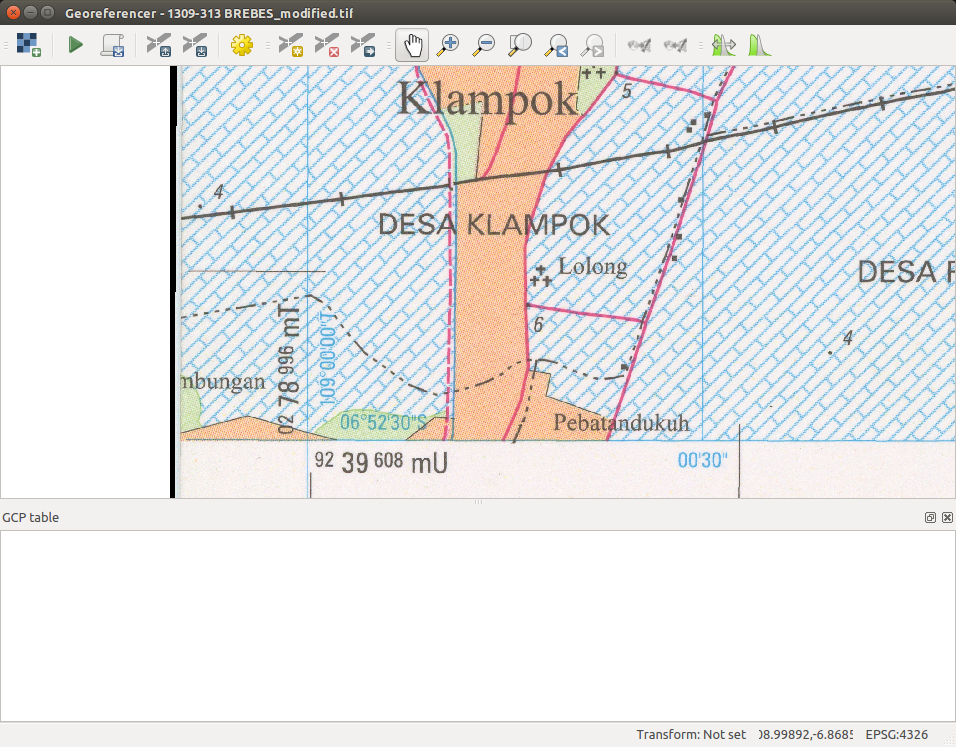
\includegraphics[scale=1]{./resources/025-icon-transformation}
    \caption{Ikon \textit{Transformation}}
    \label{fig:transformationicon}
  \end{figure}
  
  \item Setelah itu akan muncul jendela seperti pada gambar \ref{fig:transformationwin}.
  
  \begin{figure}[H]
    \centering
    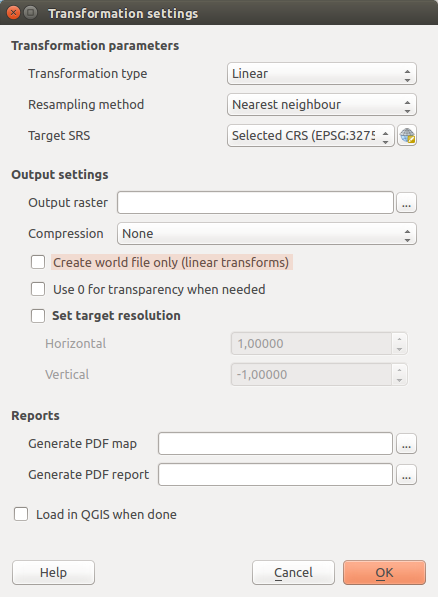
\includegraphics[width=1\textwidth]{./resources/026-transformation-win}
    \caption{Jendela Konfigurasi \textit{Transformation}}
    \label{fig:transformationwin}
  \end{figure}
  
  Yang perlu diperhatikan adalah pada bagian \verb|Target SRS|, pilihlah proyeksi yang tepat, yaitu \textbf{WGS 84 / UTM 49S} atau dengan kode yang lain adalah \textbf{EPSG:32749}. Sedangkan hasil proyeksinya dapat disimpan dalam 2 (dua) model, yang pertama akan berbentuk \textit{file} \textit{GeoTIFF} dengan ekstensi tif, dan yang kedua adalah \textit{file} tambahan berupa informasi koordinat dari \textit{raster} yang dimuat. Sehingga, untuk model yang pertama, kita tidak perlu melakukan georeferensi kembali saat memuat \textit{file GeoTIFF} ke QGIS, sedangkan untuk model yang kedua, kita tidak perlu melakukan georeferensi kembali untuk \textit{raster} yang sudah memiliki pasangan \textit{file} berupa informasi koordinat yang dihasilkan dari georeferensi ini.
  
  \item Selanjutnya membuat titik ikat atau \textit{Ground Control Point} (GCP) pada peta tersebut, maka pilih menu \verb|Edit > Add Point|, atau klik ikon seperti pada gambar \ref{fig:addpointicon}
  
  \begin{figure}[H]
    \centering
    
\includegraphics[scale=1]{./resources/027-add-point-icon}
    \caption{Ikon Tambah Titik Ikat}
    \label{fig:addpointicon}
  \end{figure}
  
  \item Apabila ingin menghapus titik ikat yang telah dibuat dapat menggunakan ikon \textit{Delete Point} seperti pada gambar \ref{fig:deletepointicon}.
  
  \begin{figure}[H]
    \centering
    
\includegraphics[scale=1]{./resources/028-delete-point-icon}
    \caption{Ikon Hapus Titik Ikat}
    \label{fig:deletepointicon}
  \end{figure}
  
  \item Sedangkan apabila ingin menggeser / memindahkan lokasi titik ikat, dapat menggunakan \textit{Move GCP Point} dengan melakukan klik pada ikon seperti pada gambar \ref{fig:movepointicon} dan arahkan pada titik ikat yang akan dipindahkan.
  
  \begin{figure}[H]
    \centering
    
\includegraphics[scale=1]{./resources/029-move-point-icon}
    \caption{Ikon Memindahkan Titik Ikat}
    \label{fig:movepointicon}
  \end{figure}
  
  \item Untuk memulai membuat titik ikat, pertama-tama \textit{Zoom} pada keempat pojok / sudut peta RBI untuk terlebih dahulu mengetahui lokasi dan nilai koordinat dari titik ikat yang akan digunakan.
  
  \item \textit{Zoom-in} di pojok kiri atas peta seperti pada gambar \ref{fig:rbismall}, kemudian buat titik di perpotongan \textit{grid} dengan tombol \textit{Add Point}, seperti yang ditunjukkan pada gambar \ref{fig:rbigrid}.
  
  \begin{figure}[H]
    \centering
    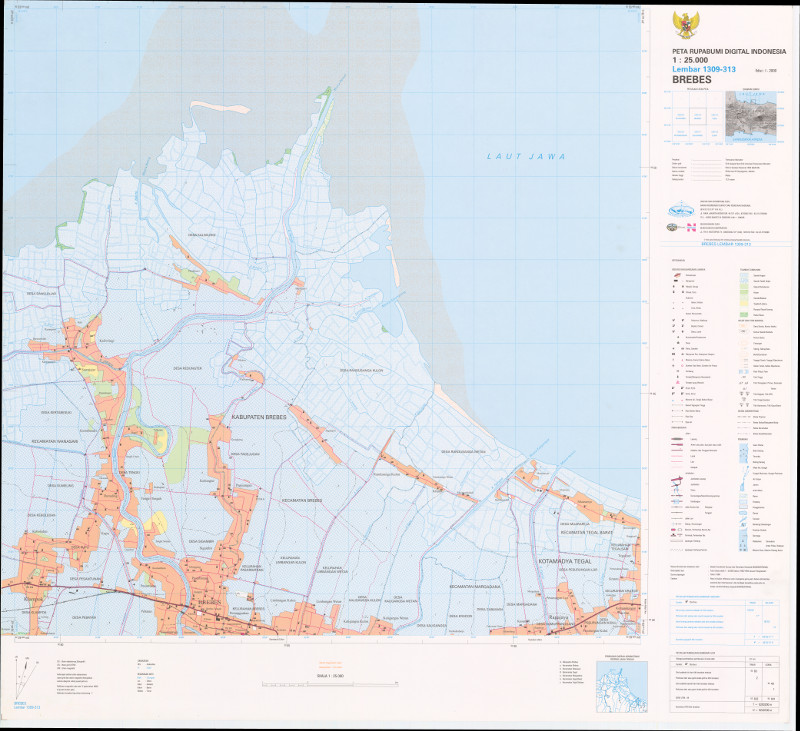
\includegraphics[width=1\textwidth]{./resources/030-rbi-brebes-resize-small}
    \caption{Peta Hasil \textit{Scan} RBI}
    \label{fig:rbismall}
  \end{figure}
  
  \begin{figure}[H]
    \centering
    \includegraphics[width=1\textwidth}{./resources/031-rbi-brebes-crop-grid}
    \caption{Hasil \textit{Zoom-in} Pojok Kiri Atas Peta RBI}
    \label{fig:rbigrid}
  \end{figure}
  
\end{enumerate}